% =====================================================================
%  panteon-mongodb-bd2 · Artículo científico (Entregable 7)
%
%  Revista : IEEE/ACM Transactions on Computational Biology and
%            Bioinformatics (TCBB)
%  Plantilla: IEEEtran, modo journal (dos columnas, 10 pt, carta)
%  Normas  : ver ../JOURNAL.md
%
%  Compilación:
%      pdflatex main
%      bibtex   main
%      pdflatex main
%      pdflatex main
% =====================================================================
\documentclass[journal]{IEEEtran}

% ------------------------- Idioma y codificación ---------------------
\usepackage[utf8]{inputenc}
\usepackage[T1]{fontenc}
\usepackage[spanish,es-noshorthands]{babel}

% ------------------------- Matemáticas y gráficos --------------------
\usepackage{amsmath}
\usepackage{amssymb}
\usepackage{graphicx}
\usepackage{booktabs}          % tablas limpias, sin líneas verticales
\usepackage{array}
\usepackage{tabularx}
\usepackage{url}
\usepackage{listings}

% ------------------------- Diagramas (TikZ) --------------------------
\usepackage{tikz}
\usetikzlibrary{shapes.multipart, positioning, arrows.meta}

% ------------------------- Hipervínculos (al final) ------------------
\usepackage[hidelinks]{hyperref}

\graphicspath{{figures/}}
\renewcommand{\arraystretch}{1.06}
\lstset{
  basicstyle=\ttfamily\footnotesize,
  breaklines=true,
  breakatwhitespace=false,
  columns=fullflexible,
  frame=single,
  framerule=0.3pt,
  xleftmargin=0pt,
  xrightmargin=0pt,
  aboveskip=6pt,
  belowskip=6pt
}

% ------------------------- Nombres traducidos ------------------------
% IEEEtran fija estos rótulos en inglés; se traducen para el manuscrito
% en español sin romper la plantilla.
\renewcommand{\abstractname}{Resumen}
\renewcommand{\IEEEkeywordsname}{Palabras clave}
\addto\captionsspanish{%
  \renewcommand{\tablename}{TABLA}%
  \renewcommand{\figurename}{Fig.}%
}

\hypersetup{
  pdftitle={Diseño y evaluación experimental de un modelo documental en MongoDB para elementos transponibles y perfiles de k-mers},
  pdfkeywords={bioinformática, bases de datos NoSQL, elementos transponibles, k-mers, modelado de datos, MongoDB},
  pdfsubject={Bases de Datos II -- Universidad Autónoma de Manizales}
}

% =====================================================================
\begin{document}

\title{Diseño y evaluación experimental de un modelo documental en MongoDB
para elementos transponibles y perfiles de \textit{k}-mers}

\author{
  Johan Andrés Villada Valencia, María Camila Prada Cortes,
  Santiago Jimenez Cotrini y Cristian Camilo Arenas Salazar%
  \thanks{Proyecto del segundo corte de Bases de Datos II, Programa de Ingeniería de
  Sistemas, Universidad Autónoma de Manizales, Manizales, Colombia. Docente: Simón
  Gaviria Orrego.}%
  \thanks{Los datos utilizados provienen de PanTEon Database v1.6.1 (Zenodo, licencia
  CC BY 4.0).}%
}

\maketitle

% ---------------------------------------------------------------------
% RESUMEN · 100--200 palabras, un solo párrafo, sin referencias ni
% ecuaciones (norma TCBB para artículo regular).
% ---------------------------------------------------------------------
\begin{abstract}
Los elementos transponibles (TEs) ocupan una fracción importante de los genomas
eucariotas y su estudio exige bibliotecas de secuencias cada vez más grandes. PanTEon
Database reúne 239.946 secuencias de animales, plantas y hongos, pero las publica como
archivos planos ---un FASTA de 946 MiB y un CSV de 363 KiB--- sin una capa de consulta que
integre secuencias, taxonomía y perfiles de \textit{k}-mers. Este trabajo diseña e
implementa un modelo documental en MongoDB de tres colecciones, con referencias por
\texttt{ObjectId}, desnormalización controlada y validación con \texttt{\$jsonSchema}. El
corpus cargado contiene 2.790 especies, 239.946 secuencias y 1.439.676 perfiles de
\textit{k}-mers (\textit{k} = 1\ldots6). Las consultas analíticas y dos preguntas propias,
resueltas con agregaciones, muestran que CLASSI concentra el 81,2\,\% de las secuencias,
que LTR, LINE y TIR reúnen el 93,4\,\% y que Plantae está dominada por LTR mientras
Animalia lo está por LINE. Comparar dos estrategias de almacenamiento muestra que agrupar
los seis perfiles reduce el espacio en disco 6,3\,\% y simplifica los índices. El modelo
se usó para exportar bibliotecas FASTA por especie y por reino sin reprocesar el archivo
de origen: 1.627 secuencias de \textit{Malus domestica} y 19.797 de Fungi.
\end{abstract}

% ---------------------------------------------------------------------
% PALABRAS CLAVE · 3--6 términos, en orden alfabético.
% ---------------------------------------------------------------------
\begin{IEEEkeywords}
bases de datos NoSQL, bioinformática, elementos transponibles, \textit{k}-mers,
modelado de datos, MongoDB
\end{IEEEkeywords}

% =====================================================================
\section{Introducción}
% =====================================================================
Los elementos transponibles (TEs) son secuencias de ADN capaces de moverse o copiarse
dentro del genoma. En algunos genomas vegetales superan el 80\,\% del contenido total y
participan en la evolución, la regulación génica y la adaptación de las especies. Se
organizan en una jerarquía de tres niveles ---clase, orden y superfamilia---, por ejemplo
\texttt{CLASSI} $\rightarrow$ \texttt{LTR} $\rightarrow$ \texttt{GYPSY} o
\texttt{CLASSII} $\rightarrow$ \texttt{HELITRON} $\rightarrow$ \texttt{HELITRON}.

Los grupos de bioinformática trabajan con bibliotecas de TEs: miles de secuencias de
muchas especies acompañadas de metadatos taxonómicos y del origen de cada biblioteca.
Para analizarlas, comparar especies o entrenar clasificadores, esas secuencias suelen
transformarse en perfiles de \textit{k}-mers: el conjunto de subsecuencias de longitud
\textit{k} que aparecen en cada secuencia y su frecuencia.

PanTEon Database publica ese material como dos archivos planos independientes
\cite{panteon2026zenodo}: un FASTA con cerca de 240.000 secuencias y un CSV con la
taxonomía y la procedencia de 2.790 especies. Esa organización, descrita en el marco de
trabajo de PanTEon \cite{orozco2026panteon}, es adecuada para distribuir el dato pero no
para explotarlo: cada consulta analítica obliga a recorrer el archivo completo, y no
existe una estructura que relacione una secuencia con su taxonomía y con su perfil de
\textit{k}-mers.

El problema crece por una razón aritmética. Con el alfabeto $\{A, C, G, T\}$ existen
$4^{k}$ \textit{k}-mers posibles, de modo que un perfil completo de \textit{k} = 1 a 6
contiene hasta $4 + 16 + 64 + 256 + 1.024 + 4.096 = 5.460$ valores. Multiplicado por
239.946 secuencias, un almacenamiento denso e ingenuo produciría del orden de
$1{,}3 \times 10^{9}$ pares clave-valor. La forma de guardar ese perfil no es un detalle
de implementación: es la decisión central del diseño.

Este trabajo aborda ese problema con un modelo documental híbrido en MongoDB y un
pipeline reproducible en Python. Los aportes son:
\begin{enumerate}
  \item un modelo de tres colecciones que integra secuencias, taxonomía y perfiles de
        \textit{k}-mers, con criterios explícitos de embebido y de referencia;
  \item un pipeline que limpia y cruza las dos fuentes, calcula atributos derivados y
        almacena los perfiles de \textit{k}-mers con una política definida para bases
        ambiguas;
  \item una evaluación experimental de dos estrategias de almacenamiento, con métricas de
        espacio en disco, tamaño de índices y estructura de los documentos.
\end{enumerate}

% =====================================================================
\section{Trabajo relacionado}
% =====================================================================
\paragraph*{Bases de datos de elementos transponibles.}
Dfam se consolidó como la base de referencia de familias de TEs, con secuencias curadas y
modelos de familia \cite{storer2021dfam}. Su fortaleza es la curación manual; su límite,
la cobertura taxonómica, que depende del esfuerzo de curaduría de cada genoma.

\paragraph*{PanTEon.}
El marco de PanTEon \cite{orozco2026panteon} amplía esa cobertura combinando cuatro
fuentes ---secuencias curadas de Dfam, secuencias de APTEdb, secuencias no curadas de Dfam
y secuencias de Ensembl--- y aplicando un proceso automático de curación con
RepeatModeler2 y MCHelper. El resultado es un conjunto \textit{cross-kingdom} (Animalia,
Plantae y Fungi) de casi 240.000 secuencias con nomenclatura estandarizada
(\texttt{>ID\#CLASE/ORDEN/SUPERFAMILIA @Especie}) y metadatos taxonómicos por especie.
PanTEon distribuye también modelos entrenados para su plataforma de clasificación.

\paragraph*{El vacío.}
Tanto Dfam como PanTEon entregan el dato, no el acceso estructurado. Ninguna de las dos
expone una interfaz que permita, por ejemplo, obtener en una sola consulta la distribución
de superfamilias por reino, o reconstruir una biblioteca \texttt{.fasta} filtrada por
especie sin volver a procesar el archivo de origen. El modelo documental reduce la
impedancia entre el dato biológico ---naturalmente jerárquico y variable--- y el esquema,
a cambio de asumir redundancia controlada. Esa es la brecha que cubre este trabajo.

% =====================================================================
\section{Materiales y métodos}
% =====================================================================

\subsection{Datos y problemas de calidad}
% ---------------------------------------------------------------------
Se trabajó con PanTEon Database v1.6.1 (Zenodo, licencia CC BY 4.0). Solo se usaron dos
archivos: el FASTA con las secuencias de los TEs, de 992.180.168 B (aproximadamente
946 MiB), y el CSV con la taxonomía y el origen por especie, de 371.391 B
(aproximadamente 363 KiB).

\paragraph*{Estructura del FASTA.}
Cada registro tiene un encabezado con tres componentes:
\begin{quote}
\ttfamily\small
>PDB00000001\#CLASSII/HELITRON/HELITRON\\
@Halicephalobus mephisto
\end{quote}
El primer componente es \texttt{id\_seq}; el segundo, la terna
\texttt{clase/orden/superfamilia}; el tercero, la especie. De los 239.946 registros,
\textbf{ninguno} presentó un encabezado malformado y \textbf{ninguno} repitió
\texttt{id\_seq}. Los identificadores no siguen un patrón único: conviven el esquema
sistemático \texttt{PDB00000001} y nombres originales de familia como
\texttt{PumCon-1.141}.

\paragraph*{Columnas del CSV.}
Se conservaron 9 de las 13 columnas: \texttt{Kingdom}, \texttt{Phylum}, \texttt{Class},
\texttt{Order}, \texttt{Family}, \texttt{Species}, \texttt{Source}, \texttt{Source 2} y
\texttt{Notes}. Se descartaron \texttt{Library?}, \texttt{Selected}, \texttt{TE\_count} y
\texttt{MCH\_Parameters} por no formar parte del alcance del proyecto.

\paragraph*{Problemas de calidad encontrados.}
La Tabla~\ref{tab:ausentes} resume los valores ausentes. Además de los nulos reales, la
columna \texttt{Order} contenía marcadores textuales de ausencia ---\texttt{No trobat},
\texttt{No order}, \texttt{No ordre NCBI}, \texttt{No Orden No trobat} y tres variantes con
\textit{incertae sedis}--- que se normalizaron a nulo, con lo cual los ausentes de
\texttt{Order} pasaron de 29 a 48.

\begin{table}[!t]
\caption{Valores ausentes en el CSV (2.790 filas).}
\label{tab:ausentes}
\centering
\footnotesize
\begin{tabular}{@{}lrr@{}}
\toprule
Columna & Nulos & \% \\
\midrule
\texttt{Phylum} & 3 & 0,11 \\
\texttt{Class} & 49 & 1,76 \\
\texttt{Order} & 29 $\rightarrow$ 48 & 1,04 $\rightarrow$ 1,72 \\
\texttt{Family} & 76 & 2,72 \\
\texttt{Notes} & 6 & 0,22 \\
\texttt{Source 2} & 2.740 & 98,2 \\
\texttt{Kingdom}, \texttt{Species}, \texttt{Source} & 0 & 0,00 \\
\bottomrule
\end{tabular}
\end{table}

Se detectaron además \textbf{columnas desalineadas en el origen}: la fila 10 tiene
\texttt{Amplistromataceae} (una familia) en \texttt{Order}; la fila 2210 tiene
\texttt{Ramicandelaberales} (un orden) en \texttt{Class}; la fila 2577 tiene
\texttt{Pleistophoridae} (una familia) en \texttt{Class}. Se conservaron sin alterar para
preservar la trazabilidad del CSV y se documentan como hallazgos de calidad del origen.

\paragraph*{Etiquetas taxonómicas fuera de nivel.}
La etiqueta \texttt{Angiosperma} se usa como \texttt{Phylum} en 418 especies y 116.441
secuencias, aunque no es una categoría de phylum. Además, tres especies (4 secuencias) no
tienen \texttt{Phylum} y una especie (2 secuencias) trae \texttt{"{} Ascomycota"} con un
espacio inicial. La consulta~3 aplica \texttt{\$trim} para unificar la categoría y reporta
\texttt{Angiosperma} como una etiqueta del CSV de origen; el dato se conserva para no
alterar la fuente.

\paragraph*{Entradas que no son especies.}
44 de las 2.790 filas de \texttt{Species} corresponden a grupos taxonómicos superiores
---\textit{Metazoa}, \textit{Mammalia}, \textit{Primates}, \textit{Rodentia},
\textit{Rattus}, \textit{Danio}, entre otros---, identificados en \texttt{Notes} como
\texttt{Dfam no especie} (34) o \texttt{No especie Repbase} (10). Se conservaron porque el
FASTA contiene secuencias de esos grupos, y se marcaron con una bandera booleana para
poder excluirlos en los rankings por especie.

\paragraph*{Cruce de las dos fuentes.}
La llave es el nombre de la especie. Se normalizó con \texttt{strip()} y se eliminaron los
puntos, que en el FASTA aparecen de forma inconsistente (\textit{Coccomyxa sp. obi} frente
a \textit{Coccomyxa sp obi}). Solo cuatro especies ---533 secuencias--- requirieron quitar
el punto: \textit{Beta vulgaris} subsp. \textit{vulgaris} (296 secuencias), \textit{Abrus
pulchellus} subsp. \textit{cantoniensis} (178), \textit{Marchantia polymorpha} subsp.
\textit{montivagans} (48) y \textit{Coccomyxa} sp. \textit{obi} (11). Tras la normalización
cruzan las \textbf{2.790 especies en ambos sentidos, sin huérfanos}, y no hay colisiones.
Para no perder el encabezado original se conserva \texttt{especie\_original} en
\texttt{species} y \texttt{sequences}; la llave sigue siendo \texttt{especie}.

\paragraph*{Bases ambiguas.}
El 22,85\,\% de las secuencias (54.837) contiene al menos una \texttt{N}, aunque el
porcentaje medio de \texttt{N} por secuencia es de 0,379\,\%. Se adoptó la política de
\textbf{descartar toda ventana de longitud \textit{k} que contenga un carácter distinto de
$\{A, C, G, T\}$}, y registrar el número de ventanas válidas para poder expresar el perfil
como frecuencia y no solo como conteo.

\subsection{Modelo de datos y decisiones de diseño}
\label{sec:modelo}
% ---------------------------------------------------------------------
El modelo es una arquitectura documental híbrida de tres colecciones unidas por
\texttt{\_id}:
\begin{center}
\texttt{species} (2.790) $\xrightarrow{1:N}$ \texttt{sequences} (239.946)
$\xrightarrow{1:N}$ \texttt{kmers} ($\leq$ 1.439.676).
\end{center}

\paragraph*{\texttt{species}.}
Un documento por especie, con la taxonomía y el origen de la biblioteca embebidos. Campos:
\texttt{especie} (índice único), \texttt{especie\_original}, \texttt{es\_especie},
\texttt{taxonomy.\{kingdom, phylum, tax\_class, tax\_order, family\}} y
\texttt{library\_origin.\{source, source\_2, notes\}}. \texttt{especie} es la llave normalizada;
\texttt{especie\_original} conserva el nombre del FASTA para la exportación.

\paragraph*{\texttt{sequences}.}
Un documento por secuencia. Además de \texttt{id\_seq} (único), \texttt{secuencia} y
\texttt{metrics.\{longitud, n\_count, gc\_count, pct\_n, pct\_gc\}}, incluye \texttt{species\_id} como
referencia y tres campos desnormalizados: \texttt{especie}, \texttt{especie\_original} y
\texttt{kingdom}. Es el patrón de \textit{extended reference}: la referencia permite el
\texttt{\$lookup} de la consulta~12 y la desnormalización evita pagarlo en las consultas
por reino y en la exportación \texttt{.fasta}.

\paragraph*{\texttt{kmers}.}
Un documento por secuencia y por \textit{k}, con \texttt{sequence\_id}, \texttt{id\_seq},
\texttt{k}, \texttt{valid\_windows} y \texttt{counts}. \texttt{counts} es un diccionario
\textbf{disperso}: solo contiene los \textit{k}-mers con conteo mayor que cero.

\begin{figure*}[t]
\centering
\begin{tikzpicture}[
  font=\footnotesize\ttfamily,
  coll/.style={
    rectangle split, rectangle split parts=2,
    draw=black!75, rounded corners=3pt, line width=0.7pt,
     rectangle split part fill={black!8, white},
    text width=5.1cm, align=left, inner sep=4pt,
    execute at begin node={\setlength{\rightskip}{0pt}}
  },
  refarrow/.style={-{Latex[length=2.5mm, width=2mm]}, thick, draw=black!80}
]

% Colección 1: species
\node[coll] (species) {
  \textbf{species} \hfill \normalfont\scriptsize (2.790 docs)
  \nodepart{second}
  \_id: ObjectId \hfill \textbf{[PK]}\\
  especie: string \hfill \textbf{[UK]}\\
  es\_especie: bool\\
  especie\_original: string\\
  \textbf{taxonomy:} \{ \hfill \textit{[embedded]}\\
  \quad kingdom: string\\
  \quad phylum: string | null\\
  \quad tax\_class: string | null\\
  \quad tax\_order: string | null\\
  \quad family: string | null \}\\
  \textbf{library\_origin:} \{ \hfill \textit{[embedded]}\\
  \quad source: string\\
  \quad source\_2: string | null\\
  \quad notes: string | null \}
};

% Colección 2: sequences
\node[coll, right=0.9cm of species] (sequences) {
  \textbf{sequences} \hfill \normalfont\scriptsize (239.946 docs)
  \nodepart{second}
  \_id: ObjectId \hfill \textbf{[PK]}\\
  id\_seq: string \hfill \textbf{[UK]}\\
  species\_id: ObjectId \hfill \textbf{[FK]}\\
  especie: string \hfill \textit{[ext. ref]}\\
  especie\_original: string\\
  kingdom: string \hfill \textit{[ext. ref]}\\
  \textbf{te\_classification:} \{ \hfill \textit{[embedded]}\\
  \quad clase\_fasta: string\\
  \quad orden\_fasta: string\\
  \quad superfamilia\_fasta: string \}\\
  \textbf{metrics:} \{ \hfill \textit{[embedded]}\\
  \quad longitud: int\\
  \quad n\_count, gc\_count: int\\
  \quad pct\_n, pct\_gc: double \}\\
  secuencia: string
};

% Colección 3: kmers
\node[coll, right=0.9cm of sequences] (kmers) {
  \textbf{kmers} \hfill \normalfont\scriptsize (1.439.676 docs)
  \nodepart{second}
  \_id: ObjectId \hfill \textbf{[PK]}\\
  sequence\_id: ObjectId \hfill \textbf{[FK]}\\
  id\_seq: string \hfill \textbf{[UK(k)]}\\
  k: int (1..6) \hfill \textbf{[UK(k)]}\\
  valid\_windows: int\\
  \textbf{counts:} \{ \hfill \textit{[sparse dict]}\\
  \quad "<kmer>": int ($>0$)\\
  \}
};

% Relaciones 1:N
\draw[refarrow] (sequences.west) -- node[above, font=\scriptsize\sffamily] {1 : N} (species.east);
\draw[refarrow] (kmers.west) -- node[above, font=\scriptsize\sffamily] {1 : N} (sequences.east);

\end{tikzpicture}
\caption{Diagrama del modelo documental híbrido en MongoDB. Se indican las llaves primarias
(\texttt{\_id}), índices únicos (\texttt{UK}), referencias por \texttt{ObjectId}
(\texttt{FK}), campos desnormalizados bajo el patrón \textit{extended reference}
(\texttt{ext. ref}) y subdocumentos embebidos.}
\label{fig:modelo_datos}
\end{figure*}

\paragraph*{Decisiones y alternativas descartadas.}
\begin{itemize}
  \item \textit{Embebido frente a referencia.} Se evaluó guardar la taxonomía completa
        dentro de cada secuencia. Se descartó porque replica cinco campos en 239.946
        documentos y porque la taxonomía cambia por especie, no por secuencia. Se adoptó la
        referencia más tres campos desnormalizados, que cubren los patrones de acceso
        dominantes.
  \item \textit{Colección aparte frente a perfiles embebidos.} Se evaluó embeber los
        perfiles en \texttt{sequences}. Se descartó porque los perfiles son la mayor parte
        del volumen y no intervienen en las consultas analíticas ni en la exportación
        \texttt{.fasta}; mantenerlos aparte evita arrastrarlos en cada lectura. La
        comparación cuantitativa de ambas opciones es, precisamente, el experimento de la
        sección~\ref{sec:diseno_experimental}.
  \item \textit{Diccionario disperso frente a arreglo denso.} Se adoptó el diccionario
        disperso. En una secuencia corta la mayoría de los 4.096 hexámeros no aparece; un
        arreglo denso almacenaría miles de ceros por documento.
  \item \textit{Un documento por \textit{k} frente a un documento único.} Se adoptó un
        documento por \textit{k} para poder recuperar un perfil sin traer los otros cinco
        (consulta~15).
  \item \textit{Identificadores.} Se usa el \texttt{\_id} ObjectId generado por MongoDB y
        se conserva el identificador original en \texttt{id\_seq}, con índice único, como
        exige la guía.
  \item \textit{Colisión de nombres.} La clase y el orden taxonómicos del CSV se
        renombraron a \texttt{tax\_class} y \texttt{tax\_order}; la clase y el orden del elemento
        se conservan como \texttt{clase\_fasta} y \texttt{orden\_fasta}. La distinción es
        explícita en el esquema.
\end{itemize}

\paragraph*{Índices.}
La Tabla~\ref{tab:indices} lista los índices del modelo. El script
\path{database/indices.js} los crea; la verificación con
\texttt{explain("executionStats")} se ejecuta en la instancia con datos
(README \S6.5). La evaluación experimental creó \texttt{\{id\_seq: 1, k: 1\}} y
\texttt{\{k: 1, valid\_windows: 1\}} sobre \texttt{kmers}; los índices de
\texttt{species} y \texttt{sequences} quedan definidos en el script y no modifican el
modelo de datos.

\begin{table*}[t]
\caption{Índices definidos y consulta que los justifica.}
\label{tab:indices}
\centering
\footnotesize
\begin{tabularx}{\textwidth}{@{}l l X@{}}
\toprule
Colección & Índice & Consulta que lo justifica \\
\midrule
\texttt{species} & \texttt{\{especie: 1\}} único & 12, 13 \\
\texttt{species} & \texttt{\{taxonomy.kingdom: 1\}} & 3, 6 \\
\texttt{sequences} & \texttt{\{id\_seq: 1\}} único & 8, 15 \\
\texttt{sequences} & \texttt{\{species\_id: 1\}} & 2, 4, 9, 12 \\
\texttt{sequences} & \texttt{\{especie: 1\}} & 2, 10 \\
\texttt{sequences} & \texttt{\{kingdom: 1\}} & 3, 6, 7, 11 \\
\texttt{sequences} & \texttt{\{te\_classification.\allowbreak clase\_fasta: 1\}} & 1, 5 \\
\texttt{sequences} & \texttt{\{te\_classification.\allowbreak orden\_fasta: 1\}} & 1, 5, 6 \\
\texttt{sequences} & \texttt{\{te\_classification.\allowbreak superfamilia\_fasta: 1\}} & 1, 5, 9 \\
\texttt{kmers} & \texttt{\{id\_seq: 1, k: 1\}} único & 15 \\
\texttt{kmers} & \texttt{\{k: 1, valid\_windows: 1\}} & Q3 de la evaluación experimental (\textit{k} = 6, ventanas $>$ 1.500) \\
\texttt{kmers} & \texttt{\{sequence\_id: 1\}} & \texttt{\$lookup} de la Fig.~\ref{fig:heatmap} (\texttt{kmers} $\rightarrow$ \texttt{sequences}) \\
\bottomrule
\end{tabularx}
\end{table*}

\paragraph*{Validación de esquema (\texttt{\$jsonSchema}).}
La validación está definida en \path{database/schema_validation.py} y se aplica con
\texttt{collMod} sobre las tres colecciones, con nivel estricto
(\texttt{validationLevel: "strict"}) y acción de rechazo
(\texttt{validationAction: "error"}), de modo que cualquier inserción o actualización que
incumpla las reglas sea abortada. En \texttt{species} y \texttt{sequences} se restringen
los campos obligatorios ---incluido \texttt{especie\_original}---, los tipos BSON
(\texttt{objectId}, \texttt{string}, \texttt{bool}, \texttt{int}, \texttt{long},
\texttt{double}), los dominios cerrados mediante \texttt{enum} (\texttt{kingdom}
$\in$ \{Animalia, Plantae, Fungi\}, \texttt{source} $\in$ \{Dfam, RM2+MCH\} y
\texttt{clase\_fasta} $\in$ \{CLASSI, CLASSII\}) y las cotas numéricas (\texttt{longitud}
$\geq$ 1 y porcentajes en $[0, 100]$). Se admite \texttt{["string", "null"]} únicamente
en los seis campos del CSV que presentan valores ausentes (\texttt{phylum},
\texttt{tax\_class}, \texttt{tax\_order}, \texttt{family}, \texttt{source\_2} y \texttt{notes}). En
\texttt{kmers} se valida la cabecera del documento (\texttt{sequence\_id}, \texttt{id\_seq},
\textit{k} $\in$ [1, 6] y \texttt{valid\_windows} $\geq$ 0) y se declara \texttt{counts} como
un \texttt{object} abierto, dado que el diccionario disperso solo almacena las llaves con
conteo mayor que cero. La migración \path{database/migrar_especie_original.py} se
ejecuta antes de aplicar el validador. El script termina con
\texttt{db.validate\_collection} para cada colección y reporta \texttt{valid=true} cuando
el esquema es consistente con los documentos existentes. \textbf{Estado:} el script se
ejecuta con la base cargada (README \S6.5); no modifica los documentos ni requiere
recalcular los \textit{k}-mers.

\subsection{Pipeline de procesamiento}
% ---------------------------------------------------------------------
El pipeline se implementó en Python con \texttt{pandas}, \texttt{biopython} y
\texttt{pymongo}, y se ejecutó en local con Anaconda y Jupyter.
\begin{enumerate}
  \item \textbf{Lectura y validación del FASTA.} Se recorre con \texttt{SeqIO}, se separa
        el encabezado en sus tres componentes y se valida que todos los registros tengan la
        estructura esperada. El resultado de la validación es un reporte de
        inconsistencias, no un filtrado silencioso.
  \item \textbf{Limpieza del CSV.} Selección de las nueve columnas, normalización de la
        llave y conversión de marcadores de ausencia a nulo.
  \item \textbf{Cruce.} Unión por nombre de especie normalizado, con reporte de huérfanos
        en ambos sentidos.
  \item \textbf{Atributos derivados.} Longitud, conteo de \texttt{N}, conteo de
        \texttt{G}+\texttt{C} y sus porcentajes.
  \item \textbf{Cálculo de \textit{k}-mers.} Para cada secuencia se ejecutan seis ventanas
        deslizantes independientes, una por cada valor de \textit{k} entre 1 y 6. Se acepta
        una ventana solo si todos sus caracteres pertenecen a $\{A, C, G, T\}$; el filtro
        cubre el alfabeto completo, no solo la ausencia de \texttt{N}. Los conteos se
        acumulan en un diccionario y el número de ventanas aceptadas se conserva en
        \texttt{valid\_windows}, que actúa como denominador para expresar el perfil como
        frecuencia.
  \item \textbf{Carga.} Inserción por lotes de 5.000 secuencias con \texttt{insert\_many},
        escribiendo de forma simultánea en \texttt{sequences} y en \texttt{kmers}. La carga
        es idempotente en el sentido operativo: al inicio se eliminan las tres colecciones,
        de modo que una re-ejecución reproduce el estado sin duplicados.
\end{enumerate}

\paragraph*{Estado de la implementación.}
La carga se ejecutó completa sobre el corpus entero y quedaron \textbf{2.790 documentos en
\texttt{species}, 239.946 en \texttt{sequences} y 1.439.676 en \texttt{kmers}}, es decir,
exactamente seis documentos de \textit{k}-mers por secuencia. El cálculo de \textit{k}-mers
se hace en Python puro con una pasada por cada valor de \textit{k}; esa etapa domina el
costo del pipeline.

\subsection{Diseño experimental}
\label{sec:diseno_experimental}
% ---------------------------------------------------------------------
Se comparan dos formas de organizar los perfiles de \textit{k}-mers, ambas sobre el corpus
completo y en la misma máquina:
\begin{itemize}
  \item \textbf{Estrategia A (modelo adoptado):} un documento por secuencia y por
        \textit{k} en la colección \texttt{kmers}. Cada documento repite
        \texttt{sequence\_id}, \texttt{id\_seq} y \textit{k}.
  \item \textbf{Estrategia B (variante medida):} un documento por secuencia que agrupa los
        seis perfiles en un arreglo \texttt{perfiles\_k}, en una colección separada.
\end{itemize}
B reduce el número de documentos de 1.439.676 a 239.946 sin mover los perfiles a la
colección de secuencias. La alternativa de embeberlos en \texttt{sequences} no forma parte
de esta comparación.

\paragraph*{Protocolo.}
La estrategia B se construye desde \texttt{kmers} con una agregación \texttt{\$out} que
agrupa por \texttt{sequence\_id}; ambas estrategias quedan sobre el corpus completo y con los
mismos documentos de origen. La comparación se hace con \texttt{db.collection.stats()}.
El notebook \texttt{03} registra además, con una corrida de calentamiento y tres
repeticiones, la mediana de \texttt{executionTimeMillis} y los documentos y llaves
examinados con y sin índice para tres consultas representativas (Q1, perfil puntual; Q2,
perfil completo de una secuencia; Q3, filtro por tamaño). Este artículo reporta la
comparación de espacio, que es la que permite decidir entre A y B; los planes de ejecución
completos quedan en el notebook.

\paragraph*{Entorno.}
La corrida se hizo sobre MongoDB 9.0.4 con las \textit{Database Tools} 100.19.1, en una
sola máquina con almacenamiento local. El equipo es un AMD Ryzen 3 3200G (4 núcleos y 4
hilos, 3,6 GHz), con 16 GB de RAM (2 $\times$ 8 GB DDR4-2666), dos discos HDD SATA de 1 TB
y Windows 10 Pro de 64 bits (build 19045).

\paragraph*{Métricas.}
\begin{enumerate}
  \item \texttt{storageSize}: espacio de los documentos.
  \item \texttt{totalIndexSize}: espacio de los índices.
  \item \texttt{avgObjSize}: tamaño promedio del documento.
  \item Espacio total: suma de datos e índices.
\end{enumerate}

% =====================================================================
\section{Resultados}
% =====================================================================

\subsection{Caracterización del conjunto de datos}
\label{sec:caracterizacion}
% ---------------------------------------------------------------------
Los conteos de esta sección se obtuvieron en la exploración con \texttt{pandas} y se
\textbf{reprodujeron después con agregaciones sobre la base cargada en MongoDB}; las cifras
coinciden de forma exacta con las de la consulta~1
(sección~\ref{sec:consultas}), de modo que ya son resultados del modelo y no solo de los
archivos de origen.

\begin{table}[!t]
\caption{Composición por reino y por origen de la biblioteca.}
\label{tab:composicion}
\centering
\footnotesize
\begin{tabular}{@{}lrr@{}}
\toprule
Reino & Especies & \% \\
\midrule
Fungi & 1.559 & 55,9 \\
Animalia & 780 & 28,0 \\
Plantae & 451 & 16,2 \\
\bottomrule
\end{tabular}

\vspace{4pt}
\scriptsize
\setlength{\tabcolsep}{2pt}
\begin{tabular}{@{}lrrrr@{}}
\toprule
Origen & Especies & Secuencias & Sec./especie & Longitud media (pb) \\
\midrule
Dfam & 386 & 31.592 & 81,84 & 1.653,8 \\
RM2+MCH & 2.404 & 208.354 & 86,67 & 4.375,5 \\
\bottomrule
\end{tabular}
\end{table}

La Tabla~\ref{tab:composicion} resume la composición por reino y por origen. El corpus
contiene \textbf{65 superfamilias} distintas. En 21.544 secuencias (8,98\,\%) la
superfamilia repite el orden, es decir, no hay un nivel específico asignado; ese
subconjunto debe interpretarse con cautela en cualquier análisis por superfamilia.

\begin{table}[!t]
\caption{Clase y orden del elemento transponible (239.946 secuencias).}
\label{tab:clase_orden}
\centering
\footnotesize
\setlength{\tabcolsep}{3pt}
\begin{tabular}{@{}lrrlr@{}}
\toprule
Clase & Secuencias & \% & Orden & Secuencias \\
\midrule
CLASSI & 194.774 & 81,2 & LTR & 119.368 \\
CLASSII & 45.172 & 18,8 & LINE & 68.382 \\
 & & & TIR & 36.471 \\
 & & & HELITRON & 5.075 \\
 & & & SINE & 3.634 \\
 & & & MITE & 3.456 \\
 & & & DIRS & 2.933 \\
 & & & PLE & 344 \\
 & & & RETROPOSON & 113 \\
 & & & CRYPTON & 112 \\
 & & & MAVERICK & 58 \\
\bottomrule
\end{tabular}
\end{table}

\begin{table}[!t]
\caption{Métricas de las secuencias.}
\label{tab:metricas}
\centering
\footnotesize
\begin{tabular}{@{}lrrrr@{}}
\toprule
Métrica & Media & Desv. est. & Mín. & Máx. \\
\midrule
\%GC & 43,02 & 7,54 & 11,03 & 78,90 \\
\%N & 0,379 & 1,186 & 0,00 & 50,06 \\
\bottomrule
\end{tabular}
\end{table}

La Tabla~\ref{tab:metricas} resume las métricas de las secuencias. Secuencias con al menos
una \texttt{N}: \textbf{54.837 (22,85\,\%)}. La longitud media es de 4.017 pb, con mínimo
de 81 y máximo de 19.926; por clase, CLASSI promedia 4.453 pb y CLASSII 2.137 pb
(consulta~5).

\paragraph*{Relación entre las dos fuentes.}
El promedio global es de 86,0 secuencias por especie (239.946 / 2.790). Al separar por
\texttt{library\_origin.source} aparecen dos perfiles distintos: RM2+MCH aporta el 86,8\,\% de
las secuencias y casi todas las especies; Dfam aporta el 13,2\,\% restante y sus secuencias
son, en promedio, 2,6 veces más cortas (Tabla~\ref{tab:composicion}). La diferencia de
longitud está confundida con el reino ---Dfam es 99,88\,\% Animalia---, así que no se
interpreta como un efecto puro de la fuente. La comparación de composición por orden se
desarrolla en la pregunta propia~1 (sección~\ref{sec:preguntas}).

\subsection{Consultas analíticas}
\label{sec:consultas}
% ---------------------------------------------------------------------
Las consultas 1--15 se implementaron como funciones en
\path{notebooks/consultas_analiticas.py} y sus resultados se calcularon sobre el
respaldo completo de la base; el notebook \texttt{02} conserva, para cada una, la pregunta,
el código y la interpretación. Las consultas 1--13 y 15 ofrecen un modo de muestreo con
\texttt{\$sample} sobre 5.000 documentos, que sirve para validar la lógica antes de lanzar
la versión completa; la consulta~14 se ejecuta sobre toda la base porque un control de
integridad sobre una muestra no prueba la ausencia de huérfanos. Los pipelines usan
\texttt{\$facet} para resolver en una sola pasada las agrupaciones que comparten la misma
etapa de filtrado y proyección, y \texttt{allowDiskUse} para no depender de la memoria
disponible.

\begin{table*}[t]
\caption{Resultado principal de cada consulta sobre la base completa.}
\label{tab:consultas}
\centering
\footnotesize
\begin{tabularx}{\textwidth}{@{}r >{\raggedright\arraybackslash}p{3.3cm} X@{}}
\toprule
\# & Consulta & Resultado principal \\
\midrule
1 & TEs por clase, orden y superfamilia & 239.946 secuencias; CLASSI 194.774 (81,2\,\%); LTR 119.368; COPIA 50.849 \\
2 & TEs por especie y clasificación & 4.642 combinaciones especie--clase; máximo \textit{Malus domestica}/CLASSI con 1.280 \\
3 & Comparación entre reinos y \textit{phyla} & 27 combinaciones por reino y 188 por \textit{phylum}; Animalia CLASSI/LINE 44.477 \\
4 & Especies con más y menos TEs & 2.746 especies; máximo \textit{Malus domestica} 1.627; mínimo varias con una sola secuencia \\
5 & Longitud por nivel taxonómico & CLASSI 4.453 pb (81--19.926); CLASSII 2.137 pb (100--18.485) \\
6 & Contenido GC por orden y reino & Fungi 46,17\,\%; Animalia 44,48\,\%; Plantae 41,25\,\%; SINE 52,97\,\% \\
7 & TEs extremos por reino & el más largo, PDB00038441 (19.926 pb, Plantae); el más corto, AllBul-4.608 (81 pb, Animalia) \\
8 & Búsqueda por \texttt{id\_seq} & PDB00000001 $\rightarrow$ \textit{Halicephalobus mephisto}, CLASSII/HELITRON \\
9 & Secuencias de una superfamilia en una especie & \textit{Puma concolor} / TRNA $\rightarrow$ 7 secuencias \\
10 & Biblioteca \texttt{.fasta} de una especie & \textit{Malus domestica} $\rightarrow$ 1.627 secuencias en \texttt{Malus\_domestica.fasta} (6,6 MB) \\
11 & Biblioteca \texttt{.fasta} de un reino & Fungi $\rightarrow$ 19.797 secuencias en \texttt{Fungi.fasta} (74,0 MB) \\
12 & Secuencias unidas a la taxonomía & 239.946 secuencias con taxón; 0 sin especie y 0 taxonomías faltantes \\
13 & Comparación por \texttt{Source} & Dfam 386 especies/31.592 secuencias (81,84 por especie); RM2+MCH 2.404/208.354 (86,67) \\
14 & Control de calidad & 0 huérfanos, 0 \texttt{id\_seq} duplicados, 0 longitudes inválidas y 0 caracteres fuera de ACGTN; 22,85\,\% con \texttt{N} \\
15 & Perfil de \textit{k}-mers de una secuencia & PDB00000001, \textit{k} = 6: 1.986 ventanas válidas y 1.253 hexámeros distintos; AAAAAA (18) y TTTAAA (15) son los más frecuentes \\
\bottomrule
\end{tabularx}
\end{table*}

\paragraph*{Composición.}
La consulta~1 reproduce exactamente los totales de la
sección~\ref{sec:caracterizacion}, lo que constituye la verificación cruzada entre la
exploración en \texttt{pandas} y el modelo cargado. Tres órdenes ---LTR, LINE y TIR---
concentran el 93,45\,\% de las secuencias, y dos superfamilias, COPIA y GYPSY, reúnen
94.812 secuencias (39,5\,\% del total). La biblioteca está, por tanto, fuertemente sesgada
hacia unos pocos grupos, y cualquier promedio global describe esa composición y no la
abundancia genómica de los TEs.

\paragraph*{Taxonomía.}
La consulta~3 resuelve el \textit{phylum} con un \texttt{\$lookup} desde \texttt{species\_id}
hacia \texttt{species.\_id}, mientras toma el reino de la referencia extendida ya presente
en \texttt{sequences}. Los tres reinos suman exactamente 239.946 secuencias, lo que
confirma que no hay referencias huérfanas; los \texttt{\$unwind} de las consultas 3 y 8 usan
\texttt{preserveNullAndEmptyArrays}, de modo que un documento sin taxón aparecería en el
conteo en lugar de desaparecer. El contraste entre reinos es el hallazgo más claro de esta
consulta: Plantae está dominada por LTR (86.049 de 119.005 secuencias, 72,3\,\%) y Animalia
por LINE (44.477 de 101.144, 44,0\,\%), con LTR en segundo lugar (25,1\,\%). Fungi ocupa
una posición intermedia, con LTR en 40,1\,\% y LINE en 31,0\,\%. La comparación se hace
sobre conteos de una biblioteca curada, no sobre anotaciones genómicas completas, de modo
que describe la composición de PanTEon y no la de los genomas de origen. Los nombres de
\textit{phylum} se conservan tal como aparecen en el CSV de origen. El caso más visible es
\texttt{Angiosperma} (418 especies, 116.441 secuencias), una etiqueta que no corresponde a
un phylum; también hay 3 especies sin phylum y una con \texttt{"{} Ascomycota"} y un
espacio inicial. La consulta~3 recorta espacios y reporta la categoría tal como llega; el
hallazgo se documenta como problema de calidad del origen.

\paragraph*{Especies.}
La consulta~4 une \texttt{sequences} con \texttt{species}, filtra
\texttt{es\_especie = true} y agrupa por el campo desnormalizado \texttt{especie}; el
\texttt{\$facet} ordena en dos sentidos. Quedan 2.746 especies y 236.184 secuencias: se
excluyen 44 entradas taxonómicas que no son especie y 3.762 secuencias. La especie con más
secuencias es \textit{Malus domestica} (1.627), seguida de \textit{Danio rerio} (1.352),
\textit{Callithrix jacchus} (1.294), \textit{Nicotiana attenuata} (1.159) y
\textit{Colobus angolensis} (1.148); \textit{Homininae}, que antes aparecía en cuarto
lugar, ya no entra en el ranking. El extremo inferior no es informativo: cientos de
especies tienen una sola secuencia y las diez mostradas son las primeras en orden
alfabético. El desempate determinista es por \texttt{especie}.

\paragraph*{Longitud y contenido GC.}
La consulta~5 muestra que CLASSI duplica en longitud promedio a CLASSII (4.453 frente a
2.137 pb), con extremos de 81 y 19.926 pb. El promedio por orden esconde asimetrías que la
mediana revela: TIR promedia 2.034 pb pero su mediana es de 1.340, mientras que LTR
promedia 5.285 pb con mediana de 5.347; MAVERICK presenta la mediana más alta (6.758 pb),
aunque sobre solo 58 registros. La consulta~6 ordena los reinos en el mismo sentido que el
tamaño de sus secuencias: Fungi presenta el mayor GC promedio (46,17\,\%), seguido de
Animalia (44,48\,\%) y Plantae (41,25\,\%). Por orden, SINE alcanza el máximo (52,97\,\%) y
MAVERICK el mínimo (40,15\,\%), aunque el segundo agrupa solo 58 secuencias. El promedio es
no ponderado por secuencia y se calcula sobre la longitud total, incluidas las \texttt{N};
como el 22,85\,\% de las secuencias contiene al menos una, el GC de ese subconjunto está
subestimado.

\paragraph*{Extremos y búsquedas puntuales.}
La consulta~7 combina \texttt{\$sort} y \texttt{\$group} con \texttt{\$first} para quedarse
con el TE más largo y el más corto de cada reino, con desempate por \texttt{id\_seq} para que
el resultado sea reproducible. Las consultas 8 y 9 ejercitan los dos caminos de acceso
previstos en el modelo: la primera necesita la taxonomía completa y paga un
\texttt{\$lookup}; la segunda busca por \texttt{especie} y \texttt{superfamilia}, que ya
están desnormalizados, y lo evita. Esa asimetría es la evidencia de uso que justifica la
referencia extendida de la sección~\ref{sec:modelo}.

\paragraph*{Exportación de bibliotecas.}
Las consultas 10 y 11 escriben el FASTA por \textit{streaming}, sin materializar la
colección completa en memoria, y reconstruyen el encabezado con \texttt{especie\_original}
para conservar los puntos que la llave normalizada elimina. La biblioteca de
\textit{Malus domestica} quedó en \path{libraries/Malus_domestica.fasta} (1.627
secuencias, 6,6 MB) y la de Fungi en \path{libraries/Fungi.fasta} (19.797 secuencias,
74,0 MB). Fungi se versiona completo porque queda por debajo del límite de 100 MB por
archivo de GitHub; las bibliotecas completas de Plantae y Animalia lo superan y se generan
localmente con la misma función. El encabezado conserva el formato
\texttt{>ID\#CLASE/ORDEN/SUPERFAMILIA @Especie}.

\paragraph*{Relación y control de calidad.}
La consulta~12 une cada secuencia con \texttt{species.\_id} y devuelve la jerarquía
completa; las 239.946 secuencias tienen taxón y no hay referencias huérfanas. La consulta~13
confirma que RM2+MCH aporta el 86,8\,\% de las secuencias y que sus TEs son 2,6 veces más
largos en promedio que los de Dfam, una diferencia confundida con el reino
(sección~\ref{sec:caracterizacion}). La consulta~14 no encontró \texttt{id\_seq} duplicados,
longitudes inválidas ni caracteres fuera de $\{A,C,G,T,N\}$. Las 44 entradas que no son
especie aportan 3.762 secuencias y se conservan en el corpus; la consulta~4 las excluye
cuando el análisis pide especies. El 22,85\,\% de las secuencias contiene al menos una
\texttt{N}, con un porcentaje medio de 0,379\,\%.

\paragraph*{Consulta 15 (perfil de \textit{k}-mers).}
La consulta~15 ya está implementada y ejecutada sobre la base completa; recupera el perfil
de una secuencia para un \textit{k} dado mediante un \texttt{\$match} por
\texttt{\{id\_seq, k\}} y un \texttt{\$project} que conserva \texttt{valid\_windows} y
\texttt{counts} sin arrastrar la secuencia completa. Para PDB00000001 con \textit{k} = 6 el
documento reporta 1.986 ventanas válidas ---es decir, una secuencia de 1.991 pb--- y 1.253
hexámeros distintos de los 4.096 posibles. El perfil está dominado por motivos ricos en A y
T: \texttt{AAAAAA} aparece 18 veces, \texttt{TTTAAA} 15, \texttt{AAAAAT} 14,
\texttt{TTTTAA} 14 y \texttt{AAATTT} 13; solo unos pocos motivos del top~20 contienen C.
Ese sesgo es coherente con el bajo contenido GC de la secuencia y con la composición de la
biblioteca, y muestra que el perfil almacenado sirve para análisis posteriores sin
recalcular los \textit{k}-mers desde el FASTA. El acceso es directo gracias al índice
\texttt{\{id\_seq, k\}}.

Los resultados de las consultas 1--15 se calcularon sobre el respaldo completo de la base.
Los índices de \texttt{kmers} sostienen la consulta~15 mediante \texttt{\{id\_seq, k\}}. La
comparación por \texttt{Source} se resume en la sección~\ref{sec:caracterizacion} y en la
pregunta propia~1; la exportación \texttt{.fasta} usa \texttt{especie\_original} para
reproducir el encabezado del archivo de origen.

\subsection{Evaluación experimental del almacenamiento}
\label{sec:benchmark}
% ---------------------------------------------------------------------
La evaluación se realizó sobre el corpus completo, con las dos estrategias construidas a
partir de los mismos documentos de \texttt{kmers}. Los valores provienen de
\texttt{collStats} y describen el espacio que ocupa cada representación.

\begin{table}[!t]
\caption{Comparación de espacio entre las dos estrategias.}
\label{tab:benchmark}
\centering
\scriptsize
\setlength{\tabcolsep}{2.5pt}
\begin{tabular}{@{}lrrr@{}}
\toprule
Métrica & A: un doc por \textit{k} & B: seis perfiles/doc & Cambio B vs. A \\
\midrule
Documentos & 1.439.676 & 239.946 & $-1.199.730$ ($-83,3$\,\%) \\
\texttt{storageSize} & 3.469,56 MB & 3.249,50 MB & $-220,06$ MB ($-6,3$\,\%) \\
\texttt{avgObjSize} & 5.644 B & 33.553 B & $+27.909$ B ($+494,5$\,\%) \\
\texttt{totalIndexSize} & 46,68 MB & 15,87 MB & $-30,81$ MB ($-66,0$\,\%) \\
Espacio total & 3.516,24 MB & 3.265,37 MB & $-250,87$ MB ($-7,1$\,\%) \\
\bottomrule
\end{tabular}
\end{table}

\paragraph*{Resultado.}
B reduce los documentos en 83,3\,\% y el espacio de datos en 6,3\,\%; sus índices ocupan
66,0\,\% menos y el espacio total baja 7,1\,\%. El documento promedio de B es mucho mayor
porque reúne los seis perfiles de una secuencia, pero esa agrupación evita repetir
\texttt{sequence\_id}, \texttt{id\_seq} y \textit{k} seis veces. La comparación matiza el
argumento de la sección~\ref{sec:modelo}: separar los perfiles ahorra lectura por perfil,
mientras que agruparlos ahorra espacio. La elección depende del patrón de acceso: A
favorece la consulta puntual de un \textit{k}; B favorece la lectura completa de la
secuencia.

\subsection{Visualización}
% ---------------------------------------------------------------------
Las cuatro figuras se generaron \textbf{directamente desde MongoDB}: la extracción de datos
está en \path{notebooks/visualizaciones.py}, la conversión a tablas y el dibujo en el
notebook \texttt{02}; todos los valores provienen de la base. Cada figura se exportó en PNG
a 300 dpi y en PDF vectorial a \path{paper/figures/}. El modo de prueba se controla con
\texttt{MODO\_PRUEBA\_FIGURAS}: con \texttt{True} se trabaja sobre 5.000 documentos y con
\texttt{False} sobre las 239.946 secuencias completas.

\begin{figure*}[t]
\centering
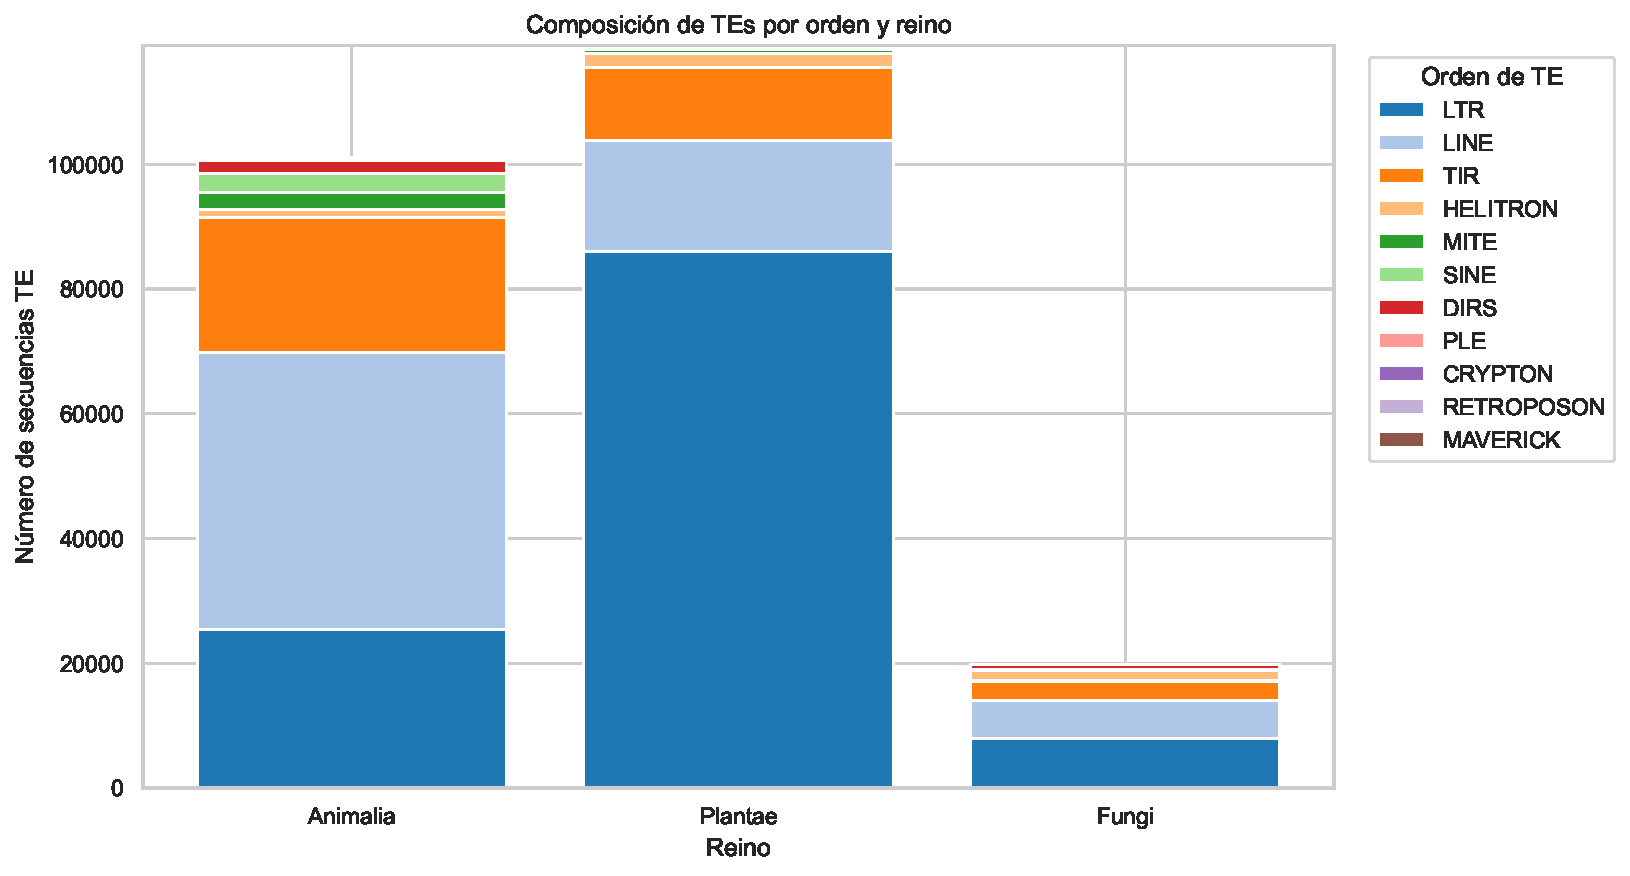
\includegraphics[width=\textwidth]{figura_1_composicion_orden_reino.pdf}
\caption{Composición de elementos transponibles por orden en Animalia, Plantae y Fungi.
Cada segmento representa un orden de TE y la altura de la barra es el número de secuencias
registradas para ese reino.}
\label{fig:composicion}
\end{figure*}

\paragraph*{Composición por orden y reino.}
La Fig.~\ref{fig:composicion} agrupa \texttt{sequences} por \texttt{kingdom} y
\texttt{te\_classification.orden\_fasta}, y representa el resultado con barras apiladas.
Plantae aporta el mayor número de registros (119.005), seguido de Animalia (101.144) y Fungi
(19.797). La composición difiere entre reinos: Plantae está dominada por LTR (86.049),
Animalia se reparte entre LINE (44.477), LTR (25.382) y TIR (21.659), y Fungi, con un
volumen mucho menor, está encabezada por LTR (7.937) y LINE (6.137).

\begin{figure}[!t]
\centering
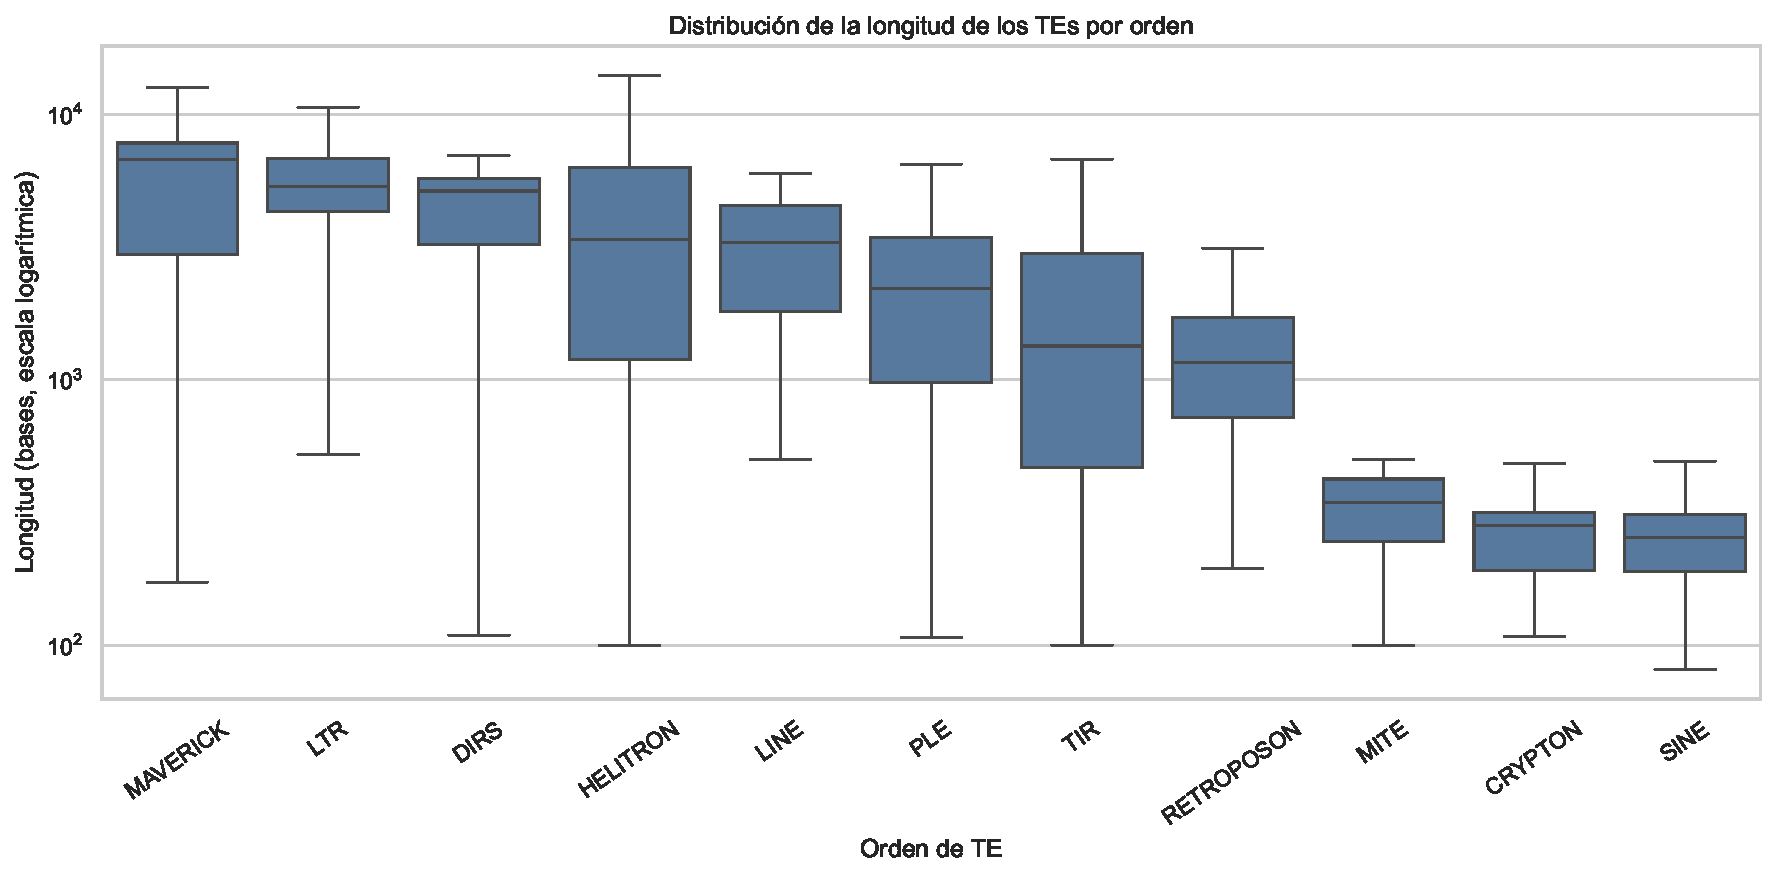
\includegraphics[width=\columnwidth]{figura_2_longitud_por_orden.pdf}
\caption{Distribución de la longitud de los elementos transponibles por orden, en escala
logarítmica.}
\label{fig:longitud}
\end{figure}

\paragraph*{Distribución de la longitud.}
La Fig.~\ref{fig:longitud} usa un diagrama de caja; el eje vertical está en escala
logarítmica porque las longitudes medianas de los órdenes difieren en más de un factor de
veinte. La figura muestra la mediana y el rango intercuartílico; los valores extremos no se
dibujan para no perder legibilidad, pero \textbf{no se eliminaron de la consulta}. La
diferencia entre media y mediana es informativa: LTR promedia 5.285 pb con mediana de 5.347,
mientras que TIR promedia 2.034 pb y tiene mediana de 1.340, señal de una cola hacia
longitudes grandes. MAVERICK presenta la mediana más alta (6.758 pb), aunque sobre 58
secuencias; el valor se calculó sobre la base completa y es el que se reporta.

\begin{figure}[!t]
\centering
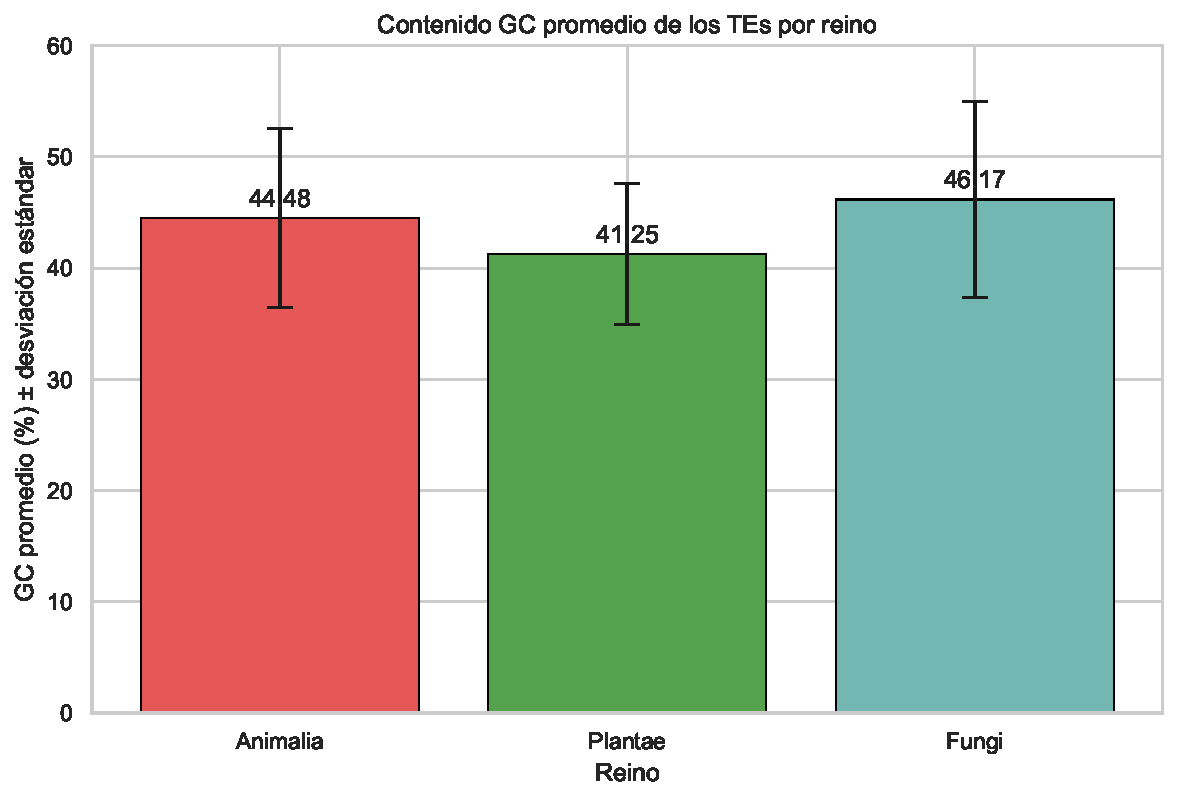
\includegraphics[width=\columnwidth]{figura_3_gc_por_reino.pdf}
\caption{Contenido GC promedio de los elementos transponibles por reino. Las barras de
error representan la desviación estándar poblacional.}
\label{fig:gc}
\end{figure}

\paragraph*{Contenido GC.}
La Fig.~\ref{fig:gc} muestra el contenido GC promedio por reino, con barras de error que
representan la desviación estándar poblacional calculada por MongoDB junto con el promedio y
el conteo: Fungi 46,17\,\% $\pm$ 8,78, Animalia 44,48\,\% $\pm$ 8,05 y Plantae
41,25\,\% $\pm$ 6,33. El promedio otorga el mismo peso a cada secuencia y no se pondera por
longitud, de modo que describe el contenido GC medio de los registros de la biblioteca y no
el de los genomas completos.

\begin{figure*}[t]
\centering
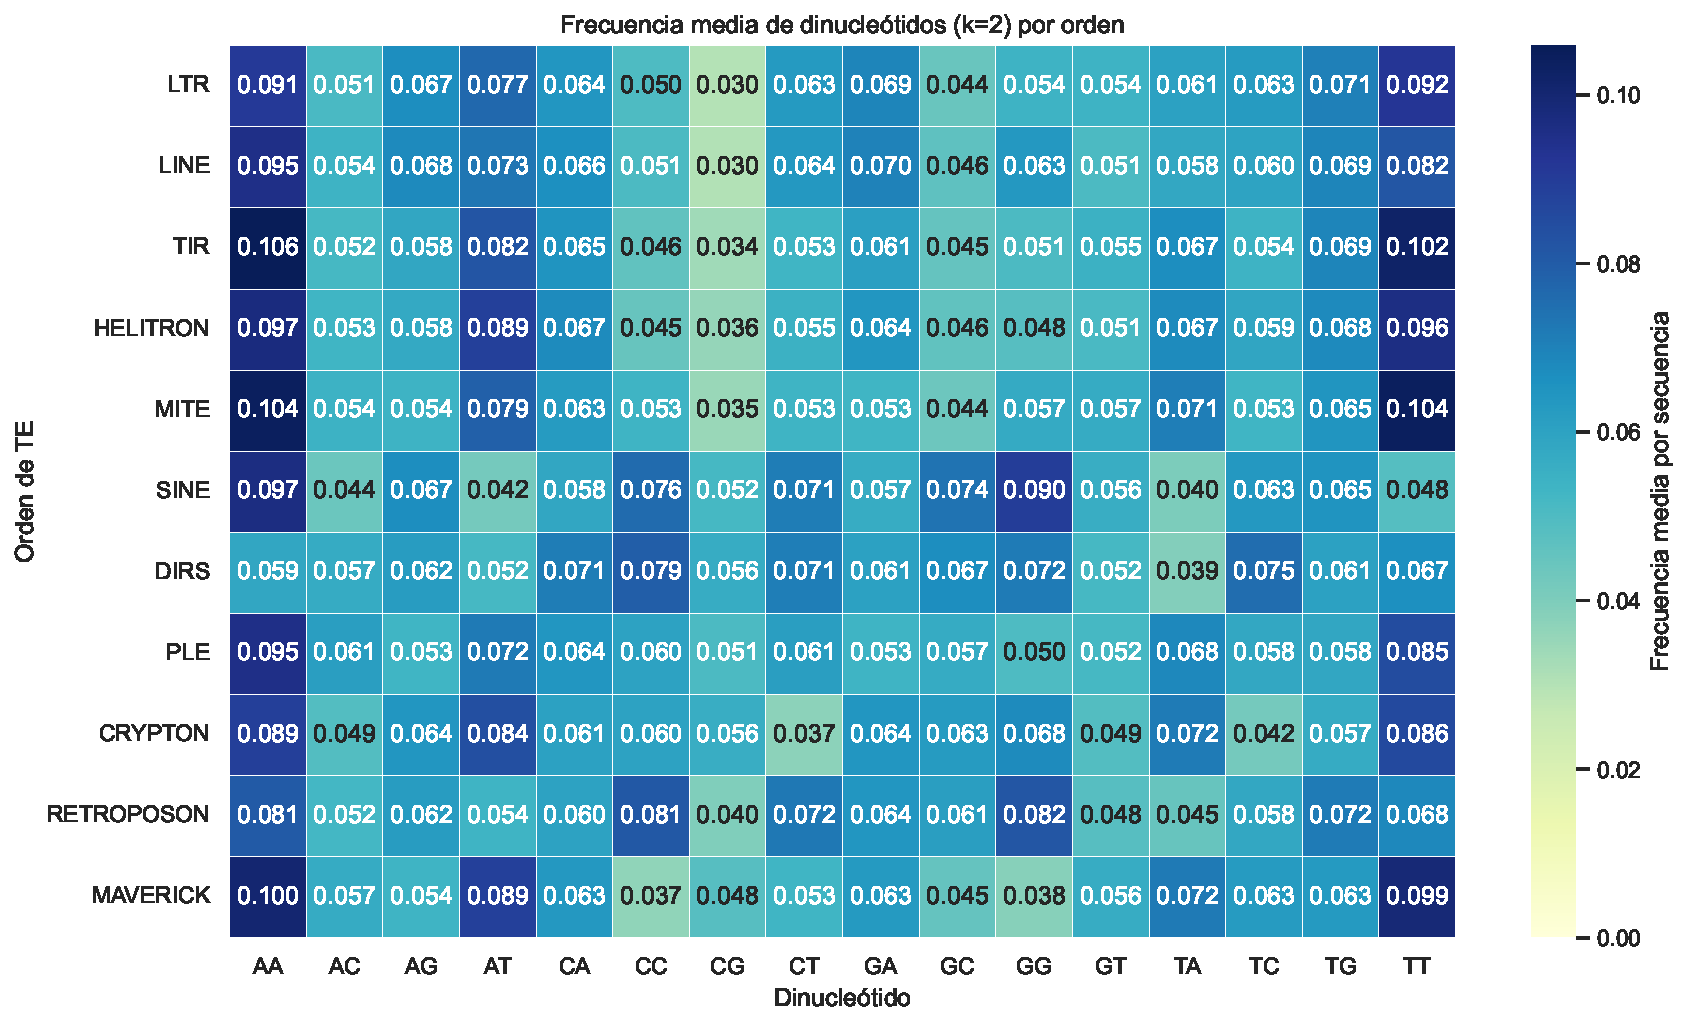
\includegraphics[width=\textwidth]{figura_4_heatmap_dinucleotidos.pdf}
\caption{Frecuencia media de los 16 dinucleótidos para \textit{k} = 2 por orden de elemento
transponible. Cada celda es el promedio de \texttt{count / valid\_windows} calculado por
secuencia.}
\label{fig:heatmap}
\end{figure*}

\paragraph*{Frecuencia de dinucleótidos.}
La Fig.~\ref{fig:heatmap} muestra la frecuencia media de los 16 dinucleótidos (\textit{k} =
2) por orden de TE. Los datos se obtienen de la colección \texttt{kmers} y el orden se
recupera con un \texttt{\$lookup} desde \texttt{kmers.sequence\_id} hacia
\texttt{sequences.\_id}. Como \texttt{counts} es un diccionario disperso, una llave ausente
significa conteo cero y no una secuencia excluida; los ceros se incorporan de forma
explícita al cálculo. Para cada secuencia se calcula la frecuencia de cada dinucleótido
como
\begin{equation}
f_{s,d} = \frac{c_{s,d}}{w_s},
\label{eq:frecuencia}
\end{equation}
donde $c_{s,d}$ es el conteo del dinucleótido $d$ en la secuencia $s$ y $w_s$ es
\texttt{valid\_windows}. Después se promedia por orden:
\begin{equation}
f_{o,d} = \frac{1}{n_o} \sum_{s \in o} f_{s,d},
\label{eq:promedio}
\end{equation}
con $o$ un orden de TE y $n_o$ el número de secuencias de ese orden. Normalizar por
secuencia antes de promediar evita que las secuencias más largas dominen el resultado, y
promediar por secuencia evita que un orden con más registros obtenga valores mayores solo
por su tamaño muestral. Omitir los ceros, en cambio, sobreestimaría la frecuencia de los
dinucleótidos presentes en pocas secuencias.

\paragraph*{Lectura conjunta.}
Las cuatro figuras describen la \textbf{biblioteca PanTEon almacenada} y no estimaciones de
abundancia genómica: los reinos y los órdenes tienen tamaños muestrales muy desiguales, y
Plantae aporta por sí sola casi la mitad del corpus (49,6\,\%). La escala logarítmica de la
Fig.~\ref{fig:longitud} oculta visualmente los valores extremos sin haberlos descartado, y
el \textit{heatmap} usa frecuencias normalizadas por secuencia, no conteos globales. Cada
una de estas decisiones se tomó para que la comparación entre grupos no dependiera del
tamaño de la muestra.

\subsection{Preguntas propias}
\label{sec:preguntas}
% ---------------------------------------------------------------------
La guía pide, además de las 15 consultas obligatorias, formular y responder al menos dos
preguntas propias. Se eligieron dos que no repiten los conteos de las consultas 1--9 y que
aprovechan las dos partes del modelo que más conviene validar: la relación
\texttt{sequences}--\texttt{species} y la colección \texttt{kmers}.

\subsubsection{Pregunta 1: ¿el origen de la biblioteca condiciona la composición de
órdenes?}
\paragraph*{Pregunta.}
¿La composición de órdenes de TEs cambia entre las bibliotecas de origen Dfam y RM2+MCH, o
ambas fuentes tienen un perfil parecido?

\paragraph*{Por qué importa.}
La consulta~13 compara cuántas especies y secuencias aporta cada \texttt{Source} y la
longitud promedio, pero no compara la composición por orden. Si Dfam y RM2+MCH tienen
proporciones distintas de LTR, LINE, TIR, etc., el \texttt{Source} es un factor de
confusión: las diferencias entre reinos o especies podrían deberse a la fuente de la
biblioteca y no a la biología. La guía pide justamente comparar Dfam contra RM2+MCH.

\paragraph*{Diseño de la consulta.}
Se une \texttt{sequences} con \texttt{species} por \texttt{species\_id}, se agrupa por
\texttt{library\_origin.source} y \texttt{orden\_fasta}, y se calcula el porcentaje dentro de cada
fuente. La agregación encadena \texttt{\$lookup}, \texttt{\$unwind} con
\texttt{preserveNullAndEmptyArrays}, dos \texttt{\$group} (uno por fuente y orden, otro por
fuente con el total), un \texttt{\$unwind} del arreglo de órdenes y un \texttt{\$project}
que calcula el porcentaje; el cálculo completo está en
\path{notebooks/preguntas_propias.py} y se ejecuta con \texttt{allowDiskUse}. Se calculó
sobre el respaldo completo de la base ---2.790 especies y 239.946 secuencias--- y se
obtuvieron 31.592 secuencias de Dfam (386 especies) y 208.354 de RM2+MCH (2.404 especies).
La composición por orden cambia de forma marcada (Tabla~\ref{tab:dfam_global}).

\begin{table}[!t]
\caption{Composición por orden dentro de cada fuente (base completa).}
\label{tab:dfam_global}
\centering
\scriptsize
\setlength{\tabcolsep}{3pt}
\begin{tabular}{@{}lrrrr@{}}
\toprule
Orden & Dfam $n$ & Dfam \% & RM2+MCH $n$ & RM2+MCH \% \\
\midrule
LTR & 10.984 & 34,77 & 108.384 & 52,02 \\
LINE & 5.660 & 17,92 & 62.722 & 30,10 \\
TIR & 11.616 & 36,77 & 24.855 & 11,93 \\
SINE & 2.270 & 7,19 & 1.364 & 0,65 \\
HELITRON & 506 & 1,60 & 4.569 & 2,19 \\
MITE & 0 & 0,00 & 3.456 & 1,66 \\
DIRS & 118 & 0,37 & 2.815 & 1,35 \\
PLE & 255 & 0,81 & 89 & 0,04 \\
CRYPTON & 64 & 0,20 & 48 & 0,02 \\
RETROPOSON & 113 & 0,36 & 0 & 0,00 \\
MAVERICK & 6 & 0,02 & 52 & 0,02 \\
\bottomrule
\end{tabular}
\end{table}

La diferencia también aparece al cruzar la fuente con el reino: Dfam es 99,88\,\% Animalia
(31.554 secuencias), 0,12\,\% Fungi (38) y 0\,\% Plantae; RM2+MCH es 57,12\,\% Plantae
(119.005), 33,40\,\% Animalia (69.590) y 9,48\,\% Fungi (19.759). Al restringir a
\texttt{es\_especie = true}, Dfam queda en LTR 36,26\,\%, TIR 34,98\,\% y LINE 18,63\,\%, de
modo que el patrón no depende de las 44 entradas taxonómicas que no son especie.

\paragraph*{Control por reino.}
Para reducir la confusión con el reino se repitió la comparación solo dentro de Animalia,
donde ambas fuentes tienen datos: Dfam aporta 31.554 secuencias y 385 especies; RM2+MCH,
69.590 y 395. El patrón se mantiene y se vuelve más nítido (Tabla~\ref{tab:dfam_animalia}).

\begin{table}[!t]
\caption{Composición por orden dentro de Animalia, por fuente.}
\label{tab:dfam_animalia}
\centering
\scriptsize
\setlength{\tabcolsep}{3pt}
\begin{tabular}{@{}lrrrr@{}}
\toprule
Orden & Dfam $n$ & Dfam \% & RM2+MCH $n$ & RM2+MCH \% \\
\midrule
LINE & 5.660 & 17,94 & 38.817 & 55,78 \\
LTR & 10.968 & 34,76 & 14.414 & 20,71 \\
TIR & 11.596 & 36,75 & 10.063 & 14,46 \\
SINE & 2.270 & 7,19 & 821 & 1,18 \\
HELITRON & 504 & 1,60 & 663 & 0,95 \\
MITE & 0 & 0,00 & 2.718 & 3,91 \\
DIRS & 118 & 0,37 & 2.007 & 2,88 \\
\bottomrule
\end{tabular}
\end{table}

Dentro de Animalia, Dfam sigue enriquecida en TIR y SINE, mientras que RM2+MCH se inclina
por LINE; LTR es mayor en Dfam que en RM2+MCH, de modo que la lectura global de ``RM2+MCH
dominada por LTR'' dependía sobre todo de Plantae.

\paragraph*{Interpretación.}
La respuesta descriptiva es sí: Dfam está enriquecida en TIR y SINE y tiene menos LINE,
mientras que RM2+MCH está dominada por LTR y LINE. Sin embargo, la fuente está fuertemente
confundida con el reino ---Dfam casi no aporta Plantae--- y por eso no se puede atribuir la
diferencia solo al origen de la biblioteca. Al restringir a Animalia, el patrón TIR/SINE
frente a LINE persiste, pero la comparación sigue sin ser aleatoria: las fuentes también
difieren en phylum y especie. El control por reino reduce una covariable importante, no
elimina todo el sesgo de selección.

\subsubsection{Pregunta 2: ¿qué dinucleótidos separan mejor los órdenes de TEs?}
\paragraph*{Pregunta.}
De los 16 dinucleótidos de \textit{k} = 2, ¿cuáles presentan la mayor diferencia de
frecuencia entre órdenes de TEs y qué órdenes tienen perfiles más parecidos?

\paragraph*{Por qué importa.}
La Fig.~\ref{fig:heatmap} muestra el perfil medio, pero no cuantifica qué dinucleótidos
aportan la separación. Esa información es la que usaría un clasificador de TEs y permite
interpretar si los órdenes se agrupan por composición (p.~ej., LTR y LINE frente a
MITE/SINE) o si el perfil es homogéneo.

\paragraph*{Diseño.}
Se reutiliza la agregación de la Fig.~\ref{fig:heatmap} para obtener la matriz
$f[\text{orden}, \text{dinucleótido}]$ (16 columnas) y se calculan dos medidas por
dinucleótido:
\begin{equation}
R_d = \max_o f[o,d] - \min_o f[o,d],
\label{eq:rango}
\end{equation}
\begin{equation}
RR_d = \frac{R_d}{\operatorname{mean}_o f[o,d]}.
\label{eq:rango_relativo}
\end{equation}
Luego se ordenan los 16 dinucleótidos por $R_d$ y $RR_d$ y se calcula la correlación de
Pearson entre los vectores de los órdenes. El cálculo de los ceros se hace igual que en la
Fig.~\ref{fig:heatmap}: una llave ausente en \texttt{counts} vale cero y se incorpora antes
de promediar.

\paragraph*{Resultado.}
Se calcularon las 16 frecuencias por secuencia y se promediaron por orden sobre las 239.946
secuencias, con 11 órdenes y 176 celdas en la matriz. Los dinucleótidos con mayor rango
absoluto entre órdenes son TT (0,0559), GG (0,0516), AA (0,0472), AT (0,0468) y CC
(0,0446). Si se normaliza por la frecuencia media, el orden cambia: GG (0,844), CC (0,768),
TT (0,661), AT (0,651) y CG (0,618) son los de mayor rango relativo
(Tabla~\ref{tab:dinucleotidos}).

\begin{table}[!t]
\caption{Dinucleótidos con mayor rango entre órdenes.}
\label{tab:dinucleotidos}
\centering
\scriptsize
\setlength{\tabcolsep}{3pt}
\begin{tabular}{@{}lrrl@{}}
\toprule
Dinucleótido & $R_d$ & $R_d$/media & Extremos (mín. $\rightarrow$ máx.) \\
\midrule
TT & 0,0559 & 0,661 & SINE 0,0484 $\rightarrow$ MITE 0,1043 \\
GG & 0,0516 & 0,844 & MAVERICK 0,0381 $\rightarrow$ SINE 0,0896 \\
AA & 0,0472 & 0,512 & DIRS 0,0586 $\rightarrow$ TIR 0,1058 \\
AT & 0,0468 & 0,651 & SINE 0,0418 $\rightarrow$ HELITRON 0,0887 \\
CC & 0,0446 & 0,768 & MAVERICK 0,0367 $\rightarrow$ RETROPOSON 0,0813 \\
\bottomrule
\end{tabular}
\end{table}

\paragraph*{Tamaño de muestra de los extremos.}
Algunos de los valores que fijan los bordes provienen de órdenes pequeños: MAVERICK tiene 58
secuencias, CRYPTON 112 y RETROPOSON 113, frente a LTR (119.368), LINE (68.382) o TIR
(36.471). MAVERICK fija el mínimo de GG y CC; RETROPOSON fija el máximo de CC; CRYPTON
aparece en la correlación negativa con DIRS ($-0,291$). No son los únicos extremos ---SINE
(3.634) y TIR (36.471) también fijan bordes---, pero los tres primeros se reportan como
descriptivos y no como estimaciones estables: con 58--113 secuencias, un cambio de unas
pocas observaciones puede mover el orden.

Las correlaciones entre perfiles separan dos bloques. TIR--HELITRON (0,982), TIR--MITE
(0,978), LTR--LINE (0,962), HELITRON--MAVERICK (0,955) y LTR--HELITRON (0,944) son las
parejas más parecidas; DIRS es el orden más distinto (correlación negativa con MAVERICK,
$-0,377$, y con CRYPTON, $-0,291$). SINE se aparta por su composición rica en GC: CG
(0,0519), GG (0,0896) y CC (0,0760) están entre sus valores más altos, mientras que AT cae
a 0,0418.

\paragraph*{Interpretación.}
Los dinucleótidos que más discriminan son los que combinan contenido GC y sesgo de cadena:
TT, GG, AA, AT y CC. La señal no es un motivo único, sino un perfil de composición; TIR,
HELITRON y MITE comparten un espacio y LTR/LINE otro, mientras que DIRS y SINE se separan.
Para un clasificador con \textit{k} = 2, estos cinco dinucleótidos son la entrada mínima
razonable; para separar DIRS o SINE harían falta \textit{k} mayores o más contexto.

% =====================================================================
\section{Discusión}
% =====================================================================
\paragraph*{Sobre el modelo.}
La decisión de separar los perfiles de \textit{k}-mers de la colección de secuencias
responde a un patrón de acceso claro: las consultas analíticas y la exportación
\texttt{.fasta} no necesitan los perfiles, y los perfiles son la mayor parte del volumen.
Mantenerlos en documentos separados evita que cada lectura de secuencia pague por un dato
que no va a usar. El costo es que la consulta~15 requiere una lectura adicional, costo que
el índice \texttt{\{id\_seq, k\}} acota. La evaluación de espacio muestra, además, que
agrupar los seis perfiles en un documento ocupa 6,3\,\% menos que separarlos; el argumento
a favor de la separación es el patrón de lectura, no el espacio.

\paragraph*{Sobre la desnormalización.}
Guardar \texttt{especie}, \texttt{especie\_original} y \texttt{kingdom} en \texttt{sequences}
replica información. Es una redundancia deliberada y acotada: dos campos de baja cardinalidad
---\texttt{especie} y \texttt{kingdom}--- que evitan un \texttt{\$lookup} en los patrones de
acceso más frecuentes, más \texttt{especie\_original}, que solo se usa al exportar la
biblioteca. La alternativa ---referencia pura--- habría hecho más simple el esquema a costa
de encarecer las consultas 3, 6, 7 y 11.

\paragraph*{Sobre los \textit{k}-mers.}
El diccionario disperso aprovecha que las secuencias de TEs son cortas en comparación con el
espacio de \textit{k}-mers: con 4.096 hexámeros posibles, una secuencia de 340 pares solo
puede activar 335 ventanas. El arreglo denso habría almacenado miles de ceros por documento.
La contrapartida es que un diccionario de llaves dinámicas no permite indexar \textit{k}-mers
individuales; si el caso de uso fuese ``buscar secuencias que contengan un \textit{k}-mer
dado'', habría que evaluar otra representación.

\paragraph*{Escalabilidad.}
Si el corpus creciera 10$\times$ (2,4 millones de secuencias), la colección \texttt{kmers}
llegaría a unos 14,4 millones de documentos; a 100$\times$, a 144 millones. El modelo
resiste estructuralmente ---las tres colecciones crecen en la misma proporción--- pero
aparecen tres necesidades: \textit{sharding} por \texttt{kingdom} o por \texttt{species\_id},
índices compuestos que cubran las agregaciones más costosas y preagregación de las
estadísticas por jerarquía, que cambian con poca frecuencia. El contraste se limita a las
mediciones de espacio de la sección~\ref{sec:benchmark}.

\paragraph*{Alcance de la evaluación.}
Las mediciones de espacio se hicieron sobre el corpus completo y no dependen de un
subconjunto. Ambas estrategias se construyeron con los mismos documentos de \texttt{kmers},
de modo que la comparación es directa. Los resultados describen este corpus y este entorno;
su generalización a volúmenes mayores requiere una nueva medición. La normalización de
especies ---que elimina puntos--- podría agrupar nombres distintos; se verificó que solo
afecta a cuatro especies (533 secuencias), que no hay colisiones y que el conteo de 2.790 no
cambia.

% =====================================================================
\section{Conclusiones}
% =====================================================================
El trabajo muestra que un modelo documental de tres colecciones ---\texttt{species},
\texttt{sequences} y \texttt{kmers}--- es suficiente para integrar las dos fuentes de
PanTEon y responder consultas analíticas sin recorrer el FASTA completo. La base cargada
contiene 2.790 especies, 239.946 secuencias y 1.439.676 documentos de perfiles. Las
consultas 1--9 reprodujeron los totales de la exploración en \texttt{pandas}: CLASSI
concentra el 81,2\,\% de las secuencias, LTR, LINE y TIR reúnen el 93,4\,\%, y la
composición cambia entre reinos (Plantae dominada por LTR, Animalia por LINE). Las consultas
10--14 completaron la exportación de bibliotecas, la relación con la taxonomía, la
comparación por fuente y el control de calidad; las bibliotecas de \textit{Malus domestica}
y Fungi conservan el encabezado original y quedaron versionadas. Las cuatro figuras se
generaron desde MongoDB y muestran que la biblioteca tiene tamaños muestrales muy
desiguales, por lo que sus promedios describen la composición de PanTEon y no la abundancia
genómica.

La separación de los perfiles de \textit{k}-mers en una colección aparte permitió resolver
la consulta~15 con un acceso directo por \texttt{\{id\_seq, k\}} y mantiene las consultas
analíticas libres del volumen de los perfiles. La comparación de las dos estrategias de
almacenamiento muestra que B reduce los documentos en 83,3\,\%, el espacio de datos en
6,3\,\% y el tamaño de los índices en 66,0\,\%; el espacio total baja 7,1\,\%. El precio es
un documento promedio mucho mayor y una lectura menos selectiva para Q1.

Las dos preguntas propias agregan un resultado que no estaba en las consultas obligatorias.
El origen de la biblioteca cambia la composición por orden ---Dfam se inclina por TIR y
SINE; RM2+MCH, por LTR y LINE en el global y por LINE dentro de Animalia---, pero la fuente
está confundida con el reino: Dfam es 99,88\,\% Animalia. Al restringir la comparación a
Animalia, el contraste TIR/SINE frente a LINE persiste, aunque la selección de especies y
phyla sigue sin ser aleatoria. En los dinucleótidos, TT, GG, AA, AT y CC son los de mayor
rango entre órdenes; TIR, HELITRON y MITE comparten perfil, LTR y LINE forman otro bloque, y
DIRS y SINE se separan. Los valores de borde y las correlaciones que dependen de MAVERICK
(58 secuencias), CRYPTON (112) y RETROPOSON (113) son descriptivos y no estimaciones
estables. Para la exportación, conservar \texttt{especie\_original} resuelve los cuatro nombres
con punto sin tocar la llave normalizada ni recargar los \textit{k}-mers.

% =====================================================================
\section*{Disponibilidad de datos y código}
% =====================================================================
Los datos provienen de PanTEon Database v1.6.1 (Zenodo, CC BY 4.0,
\url{https://doi.org/10.5281/zenodo.19372616}). El código, los notebooks y las fuentes de
este artículo están en \url{https://github.com/VilladaV/panteon-mongodb-bd2}.

El repositorio contiene los notebooks, el script de consultas, el generador de figuras,
\path{notebooks/preguntas_propias.py}, \path{database/schema_validation.py},
\path{database/migrar_especie_original.py} y \path{database/indices.js}. La secuencia
de reproducción es: descargar el FASTA y el CSV desde Zenodo, ejecutar
\path{notebooks/01_exploracion_limpieza_normalizacion_cruce.ipynb} para limpiar,
cruzar, calcular los \textit{k}-mers y cargar las tres colecciones; ejecutar los scripts de
migración, validación e índices; y ejecutar
\path{notebooks/02_consultas_y_figuras.ipynb} y
\path{notebooks/03_experimentos_diseno.ipynb}.

El respaldo completo no se versiona en el repositorio porque supera los 1,5 GB comprimidos;
está disponible en el siguiente enlace de Google Drive:
\url{https://drive.google.com/file/d/1m87QBBLpmaZzQq3VsHkd6VCQtp4fZlQU/view?usp=sharing}.
Las instrucciones para generarlo y restaurarlo están en \path{database/README.md}. Para
reproducir sin respaldo, basta con descargar el FASTA y el CSV desde Zenodo y ejecutar el
notebook~01; las consultas y las figuras se regeneran con el notebook~02, y la evaluación de
almacenamiento con el notebook~03.

% =====================================================================
\appendices
% =====================================================================
\section{Agregación de la pregunta propia 1}
\label{app:agregacion}
La consulta de la sección~\ref{sec:preguntas} se implementó con la agregación que se
reproduce a continuación. Se ejecuta sobre \texttt{sequences} con \texttt{allowDiskUse} y
produce, para cada fuente, el número de secuencias y el porcentaje de cada orden.
\begin{lstlisting}
db.sequences.aggregate([
  { $lookup: { from: "species",
               localField: "species_id",
               foreignField: "_id", as: "sp" } },
  { $unwind: { path: "$sp",
               preserveNullAndEmptyArrays: true } },
  { $group: { _id: { source: "$sp.library_origin.source",
                     orden: "$te_classification.orden_fasta" },
              n: { $sum: 1 } } },
  { $group: { _id: "$_id.source",
              total: { $sum: "$n" },
              ordenes: { $push: { orden: "$_id.orden",
                                  n: "$n" } } } },
  { $unwind: "$ordenes" },
  { $project: { _id: 0, source: "$_id",
                orden: "$ordenes.orden", n: "$ordenes.n",
                pct: { $multiply: [
                  { $divide: [ "$ordenes.n", "$total" ] },
                  100 ] } } },
  { $sort: { source: 1, pct: -1 } }
], { allowDiskUse: true })
\end{lstlisting}

\clearpage
\section{Construcción de la estrategia B}
\label{app:estrategia_b}
La variante B de la sección~\ref{sec:benchmark} se construyó desde \texttt{kmers} con una
agregación \texttt{\$out} que agrupa los seis perfiles de cada secuencia en un solo
documento. El listado siguiente reproduce la operación; el tiempo de construcción se
cronometra en el notebook~03.
\begin{lstlisting}
db.kmers.aggregate([
  { $group: {
      _id: "$sequence_id",
      id_seq: { $first: "$id_seq" },
      perfiles_k: { $push: {
        k: "$k",
        valid_windows: "$valid_windows",
        counts: "$counts"
      } }
  } },
  { $out: "kmers_estrategia_B" }
], { allowDiskUse: true })
\end{lstlisting}

% =====================================================================
% REFERENCIAS
% =====================================================================
\bibliographystyle{IEEEtran}
\bibliography{references}

\end{document}
